\documentclass{article}[12pt]
\usepackage[utf8]{inputenc}
\usepackage[T1]{fontenc}
\usepackage[ngerman]{babel}
\usepackage[dvipsnames]{xcolor}
\usepackage{lipsum}

\usepackage{amsfonts}
\usepackage[intlimits]{amsmath}
\usepackage{cite}
\usepackage{epsfig}

\usepackage[usenames,dvipsnames]{pstricks}
\usepackage{pstricks-add}
\usepackage{epsfig}
\usepackage{pst-grad} % For gradients
\usepackage{pst-plot} % For axes

\addtolength{\hoffset}{-1.5cm}
\addtolength{\textwidth}{3cm}
\usepackage{listings}
\usepackage{color}
\definecolor{mygreen}{rgb}{0,0.6,0}
\definecolor{mygray}{rgb}{0.5,0.5,0.5}
\definecolor{mymauve}{rgb}{0.58,0,0.82}
\PassOptionsToPackage{svgnames}{xcolor}
\usepackage{tcolorbox}
\usepackage{lipsum}
\tcbuselibrary{skins,breakable}
\usetikzlibrary{shadings,shadows}

\lstset{ %
  backgroundcolor=\color{white},   % choose the background color; you must add \usepackage{color} or \usepackage{xcolor}; should come as last argument
  basicstyle=\footnotesize,        % the size of the fonts that are used for the code
  breakatwhitespace=false,         % sets if automatic breaks should only happen at whitespace
  breaklines=true,                 % sets automatic line breaking
  captionpos=b,                    % sets the caption-position to bottom
  commentstyle=\color{mygreen},    % comment style
  deletekeywords={...},            % if you want to delete keywords from the given language
  escapeinside={\%*}{*)},          % if you want to add LaTeX within your code
  extendedchars=true,              % lets you use non-ASCII characters; for 8-bits encodings only, does not work with UTF-8
  frame=single,                    % adds a frame around the code
  keepspaces=true,                 % keeps spaces in text, useful for keeping indentation of code (possibly needs columns=flexible)
  keywordstyle=\color{blue},       % keyword style
  language=C,                      % the language of the code
  morekeywords={*,...},            % if you want to add more keywords to the set
  numbers=left,                    % where to put the line-numbers; possible values are (none, left, right)
  numbersep=5pt,                   % how far the line-numbers are from the code
  numberstyle=\tiny\color{mygray}, % the style that is used for the line-numbers
  rulecolor=\color{black},         % if not set, the frame-color may be changed on line-breaks within not-black text (e.g. comments (green here))
  showspaces=false,                % show spaces everywhere adding particular underscores; it overrides 'showstringspaces'
  showstringspaces=false,          % underline spaces within strings only
  showtabs=false,                  % show tabs within strings adding particular underscores
  stepnumber=1,                    % the step between two line-numbers. If it's 1, each line will be numbered
  stringstyle=\color{mymauve},     % string literal style
  tabsize=2,                       % sets default tabsize to 2 spaces
  title=\lstname                   % show the filename of files included with \lstinputlisting; also try caption instead of title
}

\usepackage{amssymb}

\newenvironment{myexampleblock}[1]{%
    \tcolorbox[beamer,%
    noparskip,breakable,
    colback=White,colframe=ForestGreen,%
    colbacklower=LimeGreen!75!White,%
    title=#1]}%
    {\endtcolorbox}

\newenvironment{myalertblock}[1]{%
    \tcolorbox[beamer,%
    noparskip,breakable,
    colback=White,colframe=Bittersweet,%
    colbacklower=Peach!75!White,%
    title=#1]}%
    {\endtcolorbox}

\newenvironment{myblock}[1]{%
    \tcolorbox[beamer,%
    noparskip,breakable,
    colback=White,colframe=RoyalBlue,%
    colbacklower=TealBlue!75!White,%
    title=#1]}%
    {\endtcolorbox}

\newenvironment{myexampleprogram}[1]{%
    \tcolorbox[beamer,%
    noparskip,breakable,
    colback=White,colframe=Goldenrod,%
    colbacklower=Yellow!75!White,%
    title=#1]}%
    {\endtcolorbox}
%--------
%\usepackage[magyar]{babel}
\title{Zufallszahlengenerator}
\begin{document}
\maketitle
Zuf\"allig generierte Zahlen sind ein wichtiges und m\"achtiges Werkzeug in der numerischen Physik. Zum Integrieren von Funktionen mit mehreren Variablen wird oft das Monte Carlo Verfahren angewendet.\\
In dieser Aufgabe werden wir einen Zufallszahlengenerator schreiben. Hierzu gibt es mehrere Methoden, die alle aus der linear Kongruenzen stammen:
\begin{equation}
I_{j+1}=a I_{j} \left( \mathrm{mod} m\right).
\label{basics}
\end{equation}
Diesen Instruktion erstellt eine neue Zufallszahl ($I_{j+1}$) aus der vorangegangenen Zahl ($I_j$). Die Qualität der Zufallszahlen 
hängt von den Eingangsparametern $(a,m)$ ab. Ein guter Zufallszahlengenerator hat große Perioden, dass hei\ss{}t der Abstand zwischen zwei gleichen
Zufallszahlen ist sehr groß. Park und Miller haben die folgenden Parameter für a und m gewählt:
\begin{equation}
a=16807, m=2^{31}-1=2147483647. 
\end{equation}
Leider ist die direkte Implementation dieses Zufallszahlengenerators mit diesen Parametern in \texttt{C} nicht möglich. Der Grund ist
dass wir keine Zahlen größer als $m$ speichern können. Glücklicherweise gibt es eine Möglichkeit das Problem umzugehen. 
Wir faktorisieren $m$:
\begin{equation}
m= aq + r; r= m \left(\mathrm{mod}a\right); q= \left[m/a\right]
\end{equation}
Damit können wir die Gleichung (\ref{basics}) auch mit ($q,r$) darstellen:
\begin{equation}
a I_j \left( \mathrm{mod} m\right)=  
\left\{ \begin{array}{rc}
a\left(I_j \mathrm{mod} q\right) -r \left[I_j/q\right] & \mathrm{wenn~es~}>0~\mathrm{ist} \\ 
a\left(I_j \mathrm{mod} q\right) -r \left[I_j/q\right] + m & \mathrm{andernfalls} \\ 
\end{array}\right.
\label{algo}
\end{equation}
hierbei ist $r=2836,q=127773$. Implementieren Sie den Zufallszahlengenerator nach eq.\ref{algo}. Ändern Sie den Algorithmus, so dass er Zahlen zwischen 0 und 1 erstellt.
Es ist wichtig unser Ergebnis zu testen. Wir müssen die Verteilung (Distribution) der Zufallszahlen testen.
Wir möchten eine gleichmäßige Verteilung erreichen. Wir werden ein Histogramm aus den Zufallszahlen machen. Wir teilen 
das Interval in $n$ Teile und z\"ahlen wie oft die Zufallszahl in jedem Interval sinkt. Erstellen Sie ein Histogramm aus 
den verfügbaren Daten und prüfen Sie wie gleichmäßig die Verteilung ist!
\\
Beispiel für die Eingabe:
\begin{lstlisting}
10000
\end{lstlisting}
Bespiel für die Ausgabe:\\
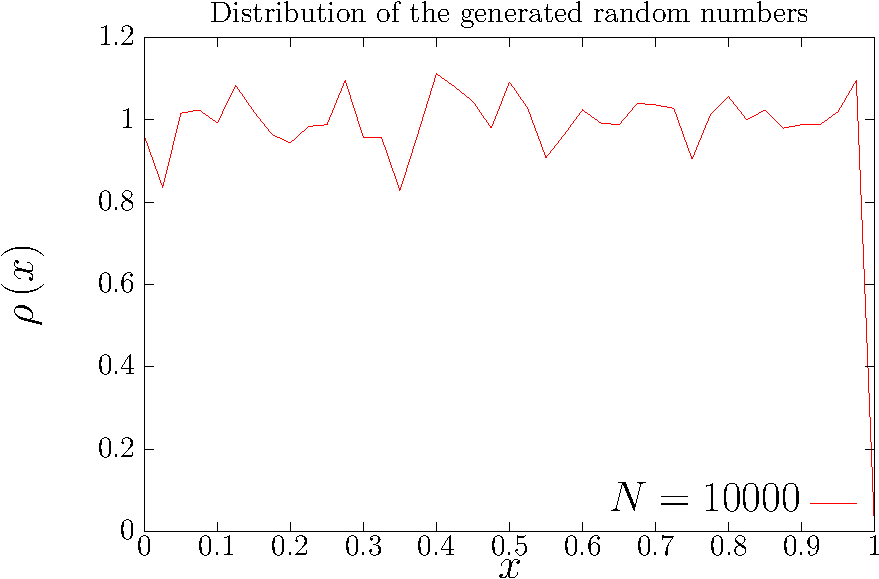
\includegraphics[width=.8\linewidth]{dist1.pdf}
\end{document}
